\documentclass{article}
\usepackage{amsmath}
\usepackage{amsfonts}
\usepackage{amssymb}

\usepackage{enumitem}

\usepackage{graphicx}

\usepackage{subcaption}

\usepackage{minted}

\usepackage{hyperref}

\begin{document}

\tableofcontents

\newpage

\section{Probability}
\subsection{Probability}
\begin{enumerate}
	\item Fill in the details of the proof of Theorem 1.8. Also, prove the monotone decreasing case.
		\begin{itemize}
			\item For the readers' convenience we restate the Continuity of Probabilities theorem. If $A_n \rightarrow A$ then $P(A_n) \rightarrow P(A)$ as $n \rightarrow \infty$. Here $A_n \rightarrow A_n$ means that either $A_n$ is monotone increasing ($A_n \subseteq A_{n + 1}$) and we define $A = \bigcup_{n = 1}^\infty A_n$, or, $A_n$ is monotone decreasing ($A_n \supseteq A_{n + 1}$) and we define $A = \bigcap_{n = 1}^\infty A_n$.
			\item We fill in the details now. First of all we want to show that $B_i \cap B_j = \emptyset$ for all $i \neq j$. Suppose without loss of generality that $i < j$ and note that $B_i \subseteq A_i$ then
			$$
			B_j = A_j \backslash \bigcup_{k = 1}^{j - 1} A_k
			$$
			and $B_i \subseteq A_i \subseteq \bigcup_{k = 1}^{j - 1}$ as such $B_i \cap B_j = \emptyset$.
			\item To see that $A_n = \bigcup_{i = 1}^n B_i$ let $x \in A_n$ then there exists a minimal $k = k(x)$ such that $x \in A_k$, i.e., for all $k' < k : x \notin A_{k'}$. Then $x \notin \bigcup_{i = 1}^{k - 1} A_i$ and therefore $x \in B_k$. Because $x$ are arbitrary it folows that $A_n \subseteq \bigcup_{i = 1}^n B_i$. On the other hand
			$$
			\bigcup_{i = 1}^n \underbrace{B_i}_{\subseteq\ A_i} \subseteq \bigcup_{i = 1}^n A_i = A_n,
			$$
			where we have used that $A_n$ is monotone increasing. The property that
			$$
			\bigcup_{i = 1}^\infty A_i = \bigcup_{i = 1}^\infty B_i
			$$
			holds is identical to the finite case, an element is part of the (countably) infinite union if there exists some minimual $i$ such that ...
			\item For the monotone decreasing case we instead want to define $B_n := A_n \backslash \bigcup_{i > n} A_i$.
		\end{itemize}
	\item Prove the statements in equation (1.1).
		\begin{itemize}
			\item This can immediately be seen by noting that $A \cup B = (A \backslash B) \cup (A \cap B) \cup (B \backslash A)$ is a disjoint union.
		\end{itemize}
	\item Let $\Omega$ be a sample space and let $A_1, A_2, \dots, $ be events. Define $B_n = \bigcup_{i = n}^\infty A_i$ and $C_n = \bigcap_{i = n}^\infty A_i$
		\begin{enumerate}
			\item Show that $(B_i)$ is monotone decreasing and that $(C_i)$ is monotone increasing.
			\item Show that $\omega \in \bigcap_{n = 1}^\infty B_n$ if and only if $\omega$ belongs to an infinite number of events $A_1, A_2, \dots$.
				\begin{itemize}
					\item Let $\omega \in \bigcap_{n = 1}^\infty B_n$ be such that $\omega$ does not belong to an infinite number of events $A_1, A_2, \dots$, i.e., there exists $N \in \mathbb{N}$ such that for all $k > N$ it follows that $\omega \notin A_k$. But then $\omega \notin B_k$ for all $k > N$ and as such does not lie in the intersection over all the $B_k$, which is a contradiction.
					\item Suppose $\omega$ lies in infinitely many $A_1, A_2, ...$. Then there exists a sequence $(A_{n_i})_{i \in \mathbb{N}}$ such that $n_i < n_{j}$ for all $i < j$ and such that $\omega \in A_{n_i}$ for all $i \in \mathbb{N}$. In that case
					$$
					\omega \in B_{n_i}
					$$
					for all $i \in \mathbb{N}$, in particular $\omega \in \cap_{i = \mathbb{N}} B_{n_i}$. Because $B_n$ is monotone decreasing the statement follows.
				\end{itemize}
			\item Show that $\omega \in \bigcup_{n = 1}^\infty C_n$ if and only if $\omega$ belongs to all the events $A_1, A_2, \dots$ except possibly a finite number of those events.
				\begin{itemize}
					\item Let $\omega \in \bigcup_{n = 1}^\infty B_n$ then there exists $n \geq 1$ such that $\omega \in B_n$. This means that $\omega \in \bigcap_{i = n}^\infty$, i.e., $\omega$ belongs to all $A_i$ where $i \geq n$.
					\item Now suppose $\omega$ belongs to all events $A_1, A_2, \dots$ except for a finite number of events. In that case there exist $N \in \mathbb{N}$ such that $\forall k \geq N : \omega \in A_k$. This means that
					$$
					\omega \in \bigcap_{i \geq k} A_i,
					$$
					i.e., $\omega \in C_k$. In particular this shows
					$$
					\omega \in C_k \subseteq \bigcup_{r \geq 1} C_r.
					$$
				\end{itemize}
		\end{enumerate}
	\item Let $\{A_i : i \in I\}$ be a collection of events where $I$ is an arbitrary index set. Show that
	$$
	\begin{aligned}
	\left( \bigcup_{i \in I} A_i \right)^c = \bigcap_{i \in I} A_i^c, && \left( \bigcap_{i \in I} A_i \right)^c = \bigcup_{i \in I} A_i^c
	\end{aligned}
	$$
	holds.

	Hint: First prove this for $I = \{1, 2, \dots, n\}$.
		\begin{itemize}
			\item I guess they want us to show it using induction in the hint, I'll just do it directly.
			$$
			\begin{aligned}
			\bigcap_i A_i^c &= \{x : \forall i : x \notin A_i\} \\
			&= \left\{x : \neg \left( \exists i : x \in A_i \right)\right\} \\
			&= \{x : \exists i : x \in A_i\}^c = \left( \bigcup_{i \in I} A_i \right)^c
			\end{aligned}
			$$
			The other direction is analogous.
		\end{itemize}
	\item Suppose we toss a fair coin until we get exactly two heads. Describe the sample space S. What is the probability that exactly k tosses are required?
	\item Let $\Omega = \{0, 1, \dots \}$. Prove that there does not exist a uniform distribution on $\Omega$ (i.e., if $P(A) = P(B)$ whenever $|A| = |B|$, then $P$ cannot satisfy the axioms of probability.)
		\begin{itemize}
			\item Note that $P(\{0\}) \neq 0$ because otherwise $P = 0$, which would mean $P$ is not a probability function. But then it follows for all $n \in \mathbb{N}$:
			$$
			P(\{0, \dots, n\}) = P\left(\bigcup_{k = 0}^n \{k\} \right) = \sum_{k = 0}^n P(\{k\}) = (n + 1)P(\{0\}) \rightarrow \infty
			$$
			for $n \rightarrow \infty$, which is a contradiction to $P(\Omega) = +1$.
		\end{itemize}
	\item Let $A_1, A_2, \dots$ be events. Show that
	$$
	\left( \bigcup_{n = 1}^\infty A_n \right) \leq \sum_{n = 1}^\infty P(A_n).
	$$
	Hint: Define $B_n = A_n \backslash \bigcup_{i = 1}^{n - 1} A_i$. Then show that the $B_n$ are disjoint and that
	$$
	\bigcup_{n = 1}^\infty A_n = \bigcup_{n = 1}^\infty B_n.
	$$
	\begin{itemize}
		\item This was basically already shown in the first exercise, the only thing we mention here is that we only have to consider the case where the series on the right hand side converges, because the left hand side is always $\leq 1$.
	\end{itemize}
	\item Suppose that $P(A_i) = 1$ for each $i$. Prove that
	$$
	P\left( \bigcap_{i = 1}^\infty A_i \right) = 1.
	$$
		\begin{itemize}
			\item Note that $P(A_i^c) = 1 - P(A_i) = 0$ and that
			$$
			P\left( \bigcap_{i = 1}^\infty A_i \right) = 1 - P\left( \bigcup_{i = 1}^\infty A_i^c \right).
			$$
			The latter can be calculated as follows:
			$$
			\begin{aligned}
			0 &\leq P\left( \bigcup_{i = 1}^\infty A_i^c \right) \\
			&\leq \sum_{i = 1}^\infty P(A_i^c) = 0
			\end{aligned}
			$$
			where we have used that probability measures are subadditive. As such $P\left( \bigcup_{i = 1}^\infty A_i^c \right) = 0$ and therefore
			$$
			P\left( \bigcap_{i = 1}^\infty A_i \right) = 1.
			$$
		\end{itemize}
	\item For fixed $B$ such that $P(B) > 0$, show that $P(\cdot|B)$ satisfies the axioms of probability.
		\begin{itemize}
			\item[Axiom 1:] Let $A$ be arbitrary then $P(A|B) = \frac{P(A, B)}{P(B)} \geq P(A, B) \geq 0$.
			\item[Axiom 2:] $P(\Omega|B) = \frac{P(\Omega, B)}{P(B)} = \frac{P(B)}{P(B)} = 1$.
			\item[Axiom 3:]
			$$
			\begin{aligned}
			P\left(\left.\bigcup_{i = 1}^\infty A_i \right| B\right) &= \frac{1}{P(B)} P\left(\bigcup_{i = 1}^\infty A_i, \right) \\
			&= \frac{1}{P(B)} \sum_{i = 1}^\infty P(A_i, B) \\
			&= \sum_{i = 1}^\infty P(A_i|B).
			\end{aligned}
			$$
		\end{itemize}
	\item You have probably heard it before. Now you can solve it rigorously. It is called the "Monty Hall Problem." A prize is placed at random behind one of three doors. You pick a door. To be concrete, let's suppose you always pick door $1$. Now Monty Hall chooses one of the other two doors, opens it and shows you that it is empty. He then gives you the opportunity to keep your door or switch to the other unopened door.Should you stay or switch? Intuition suggests it doesn't matter. The correct answer is that you should switch. Prove it. It will help to specify he sample space and the relevant events carefully. Thus write $\Omega = \{(\omega_1, \omega_2): \omega_i \in \{1,2,3\}\}$ where $\omega_1$ is where the prize is and $\omega_2$ is the door Monty opens.
		\begin{itemize}
			\item Note that $\{(1, 1), (2, 2), (3, 3)\}$ are invalid because he'll never open the door with the price. The staying strategy wins on $\{(1, 2), (1, 3)\}$, the switching strategy wins on $\{(2, 3), (3, 2)\}$. Note that this means, if $\omega_1 \neq 1$, then we are guaranteed to win. As such we win whenever $\omega_1 \in \{2, 3\}$, as such the winning probability is $2/3$ for the switching strategy.
			\item This is a pretty subtle problem, the intuition is that him opening a door does not grant new information. If $\omega_1 = 1$ then his reveal is arbitrary and we lose on switching. If $\omega_1 = 2, 3$ then he's forced to reveal the nonempty door, as such either the remaining door is the price or $\omega_1 = 1$. As such when we switch we are guaranteed to win whenever $\omega_1 = 2, 3$.
		\end{itemize}
	\item Suppose that $A$ and $B$ are independent events. Show that $A^c$ and $B^c$ are independent events.
		\begin{itemize}
			\item
			$$
			\begin{aligned}
			P(A^c, B^c) &= P((A \cup B)^c) \\
			&= 1 - P(A \cup B) \\
			&= 1 - P(A) - P(B) + P(A, B) \\
			&= 1 - P(A) - P(B) + P(A)P(B) \\
			&= (1 - P(A))(1 - P(B)) \\
			&= P(A^c)P(B^C).
			\end{aligned}
			$$
		\end{itemize}
	\item There are three cards. The first is green on both sides, the second is red on both sides and the third is green on one side and red on the other. We choose a card at random and we see one side (also chosen at random) . If the side we see is green, what is the probability that the other side is also green? Many people intuitively answer $\frac{1}{2}$. Show that the correct answer is $\frac{2}{3}$.
	\item Suppose that a fair coin is tossed repeatedly until both a head and tail have appeared at least once.
		\begin{enumerate}
			\item Describe the sample space $\Omega$.
			\item What is the probability that three tosses will be required?
		\end{enumerate}
	\item Show that if $P(A) = 0$ or $p(A) = 1$ then $A$ is independent of every other event. Show that if A is independent of itself then $P(A)$ is either $0$ or $1$.
		\begin{itemize}
			\item $P(A) = P(A, A) = P(A)P(A) = P(A)^2 \iff P(A)(P(A) - 1).$
		\end{itemize}
	\item The probability that a child has blue eyes is $1 / 4$. assume independence between children. Consider a family with $3$ children.
		\begin{enumerate}
			\item If it is known that at least one child has blue eyes, what ist he probability that at least two children have blue eyes?
				\begin{itemize}
					\item Assuming that having blue eyes is independent from the other children then the chance that none of the siblings have blue eyes is $\left(\frac{3}{4}\right)^2 = \frac{9}{16}$. As such the probability is $7 / 16$. 
				\end{itemize}
			\item If it is known that the youngest child has blue eyes, what is the probability that at least two children have blue eyes?
				\begin{itemize}
					\item While this doesn't seem intuitive this actually changes the probabilities. To see this note that in the first problem the arrangements of having at least 2 blue eyed children were $BBB$, $BBG$, $BGB$, $GBB$ where the children are ordered by age. But now we disregard the case $GBB$ as such the probability becomes smaller.
					\item The probability is then $\left(\frac{1}{4}\right)^2 + \frac{1}{4} \frac{3}{4} + \frac{3}{4}\frac{1}{4}$
				\end{itemize}
		\end{enumerate}
	\item Prove Lemma 1.14.
		\begin{itemize}
			\item
			$$
			P(A|B) = \frac{P(A, B)}{P(B)} = \frac{P(A)P(B))}{P(B)} = P(A).
			$$
			\item
			$$
			\begin{aligned}
			P(AB) &= P(A, B) \frac{P(B)}{P(B)} \\
			&= P(A|B) P(B) \\
			& = P(B|A) \frac{P(A)}{P(B)} P(B) \\
			&= P(B|A)P(A).
			\end{aligned}
			$$
		\end{itemize}
	\item Show that
	$$
	P(A, B, C) = P(A|BC)P(B|C)P(C).
	$$
	\item Suppose $k$ events form a partition of the sample space $\Omega$, i.e., they are disjoint and 
	$$
	\bigcup_{i = 1}^k A_i = \Omega.
	$$
	Assume that $P(B) > O$. Prove that if $P(A_1|B) < P(A_1)$ then $P(A_i|B) > P(A_i)$ for some $i = 2, \dots, k$.
		\begin{itemize}
			\item Suppose this statement is wrong, i.e. $P(A_1|B) < P(A_1)$ and for all $i = 2, \dots, k$ we have $P(A_i|B) \leq P(A_i)$. It then follows that
			$$
			\begin{aligned}
			\sum_{i = 1}^k P(A_i|B) &= \underbrace{P(A_1|B)}_{< P(A_1)} + \sum_{i = 2}^k \underbrace{P(A_i|B)}_{\leq P(A_i)} \\
			&< P(A_1) + \sum_{i = 1}^k P(A_i) = 1.
			\end{aligned}
			$$
			Multiplying $\sum_{i = 1}^n P(A_i|B) < 1$ by $P(B) > 0$ yields
			$$
			\sum_{i = 1}^n P(A_i|B)P(B) < P(B).
			$$
			This is a contradiction because $\sum_{i = 1}^n P(A_i|B)P(B) = \sum_{i = 1}^n P(A_i, B) = P\left(\bigcup_{i = 1}^n A_i , B\right) = P(\Omega, B) = P(B)$.
		\end{itemize}
	\item Suppose that $30\%$ of computer owners use a Macintosh, $50\%$ use Windows, and $20\%$ use Linux. Suppose that $65\%$ of the Mac users have succumbed to a computer virus, $82\%$ of the Windows users get the virus, and $50\%$ of the Linux users get the virus. We select a person at random and learn that her system was infected with the virus. What is the probability that she is a Windows user?
		\begin{itemize}
			\item Denote the operating systems by $M, W, L$ and having the virus by $V$. Using this notation we obtain $P(M) = 0.3$, $P(W) = 0.5$ and $P(L) = 0.2$. Furthermore $P(V|M) = 0.65$, $P(V|W) = 0.82$ and $P(V|L) = 0.5$ We can use the law of total probability to calculate the probability of a random person having a virus as being
			$$
			\begin{aligned}
			P(V) &= P(V, M) + P(V, W) + P(V, L) \\
			&= P(V|M)P(M) + P(V|W)P(W) + P(V|L)P(L) \\
			&= 0.65 \cdot 0.3 + 0.82 \cdot 0.5 + 0.5 \cdot 0.2 \\
			&= 0.705 = 70.5\%.
			\end{aligned}
			$$
			Now we can use Bayes' Theorem to calculate
			$$
			P(W|V) = P(V|W) \frac{P(W)}{P(V)} = 0.82 \frac{0.5}{0.705} = 0.5816 = 58.16\%
			$$
		\end{itemize}
	\item A box contains 5 coins and each has a different probability of showing heads. Let $P_1, P_2, P_3, P_4, P_5$ denote the probability of heads on each coin. Suppose that
	$$
	\begin{aligned}
	p_1 = 0,&& p_2 = 1/4,&& p_3 = 1/2,&& p_4 = 3/4,&& p_5 = 1.
	\end{aligned}
	$$
	Let $H$ denote "heads is obtained" and let $C_i$ denote the event that coin $i$ is selected.
	\begin{enumerate}
		\item Select a coin at random and toss it. Suppose a head is obtained. What is the posterior probability that coin $i$ was selected ($i = 1, ..., 5$)? In other words, find $P(C_i|H)$ for $i = 1, ..., 5$.
			\begin{itemize}
				\item Note that $P(C_i) = \frac{1}{5}$ and $P(H|C_i) = p_i$. The total probability of gettings heads is
				$$
				\begin{aligned}
				P(H) &= \sum_{i = 1}^5 P(H|C_i)P(C_i) \\
				&= \frac{1}{5} \sum_{i = 1}^5 P(H|C_i) \\
				&= \frac{1}{5} \sum_{i = 1}^5 p_i \\
				&= \frac{1}{5} (0 + 1/4 + 1/2 + 3/4 + 1) \\
				&= 0.5 = 50\%.
				\end{aligned}
				$$
				We can use Bayes' theorem to calculate
				$$
				\begin{aligned}
				P(C_i|H) &= P(H|C_i) \frac{P(C_i)}{P(H)} \\
				&= P(H|C_i) \frac{\frac{1}{5}}{0.5} \\
				&= P(H|C_i) \frac{2}{5}.
				\end{aligned}
				$$
				Using  this we obtain
				\begin{center}
				\begin{tabular}{|c|c|c|c|c|c|}
				\hline
				$i$ & 1 & 2 & 3 & 4 & 5 \\ 
				\hline
				$P(C_i|H)$ & 0 & 1/10 & 1/5 & 3/10 & 2/5 \\
				\hline
				\end{tabular}
				\end{center}
			\end{itemize}
		\item Toss the coin again. What is the probability of another head? In other words find $P(H_2|H_1)$ where $H_j$ = "heads on toss $j$."
			\begin{itemize}
				\item Suppose we have chosen the $ith$ coin then the probability of getting heads is $P(H|C_i)$. The probabilities of the individual coins have been calculated before and we just have to take the weighted sum over those.
\begin{minted}{python}
import numpy as np

mC = np.array([0, 1/10, 1/5, 3/10, 2/5])
mP = np.array([0, 0.25, 0.5, 0.75, 1])
np.dot(mC, mP)

> 0.75
\end{minted}
			\end{itemize}
		\item Find $P(C_i|B_4)$ where $B_4$ = "first head is obtained on toss $4$."
			\begin{itemize}
				\item First note that $P(C_i) = P(C_i, H_1) + P(C_i, H_1^c)$ as such
				$$
				P(C_i, H_1^c) = P(C_i) - P(C_i, H_1) = P(C_i) - P(C_i|H_1)P(H_1) = \frac{1}{5} - P(C_i|H_1) \frac{1}{2}
				$$
				as such
				\begin{center}
				\begin{tabular}{|c|c|c|c|c|c|}
				\hline
				$i$ & 1 & 2 & 3 & 4 & 5 \\ 
				\hline
				$P(C_i|H_i^c)$ & 0.2 & 0.15 & 0.1 & 0.05 & 0 \\
				\hline
				\end{tabular}
				\end{center}
				$P(H_1, H_2) = P(H_2|H_1)P(H_1) = \frac{3}{4}$
			\end{itemize}
	\end{enumerate}
	\item (Computer Experiment.) Suppose a coin has probability $p$ of falling heads up. If we flip the coin many times, we would expect the proportion of heads to be near $p$. We will make this formal later. Take $p = 0.3$ and $n = 1000$ and simulate $n$ coin flips. Plot the proportion of heads as a function of n. Repeat for $p = 0.03$.
		\begin{itemize}
			\item 
\begin{minted}{python}
import numpy as np
import matplotlib.pyplot as plt
import math

def Ex1_21(p = 0.3, n = 1000, draw = True, save = False):
    rand = np.random.random(size = 1000)
    _range = np.arange(1, n + 1)

    result = np.cumsum(rand < p) / _range

    fig, ax = plt.subplots()

    ax.plot(_range, result)

    if draw:
        plt.show()

    if save:
        # p = 0.213, n = 1000 -> 21pct_1000
        str_form = f"{math.floor(p * 100)}pct_{n}"
        fig.savefig(f"Ex1_21-{str_form}.png")

Ex1_21(p = 0.3, draw = True, save = True)
Ex1_21(p = 0.03, draw = True, save = True)
\end{minted}
		\begin{tabular}{cc}
			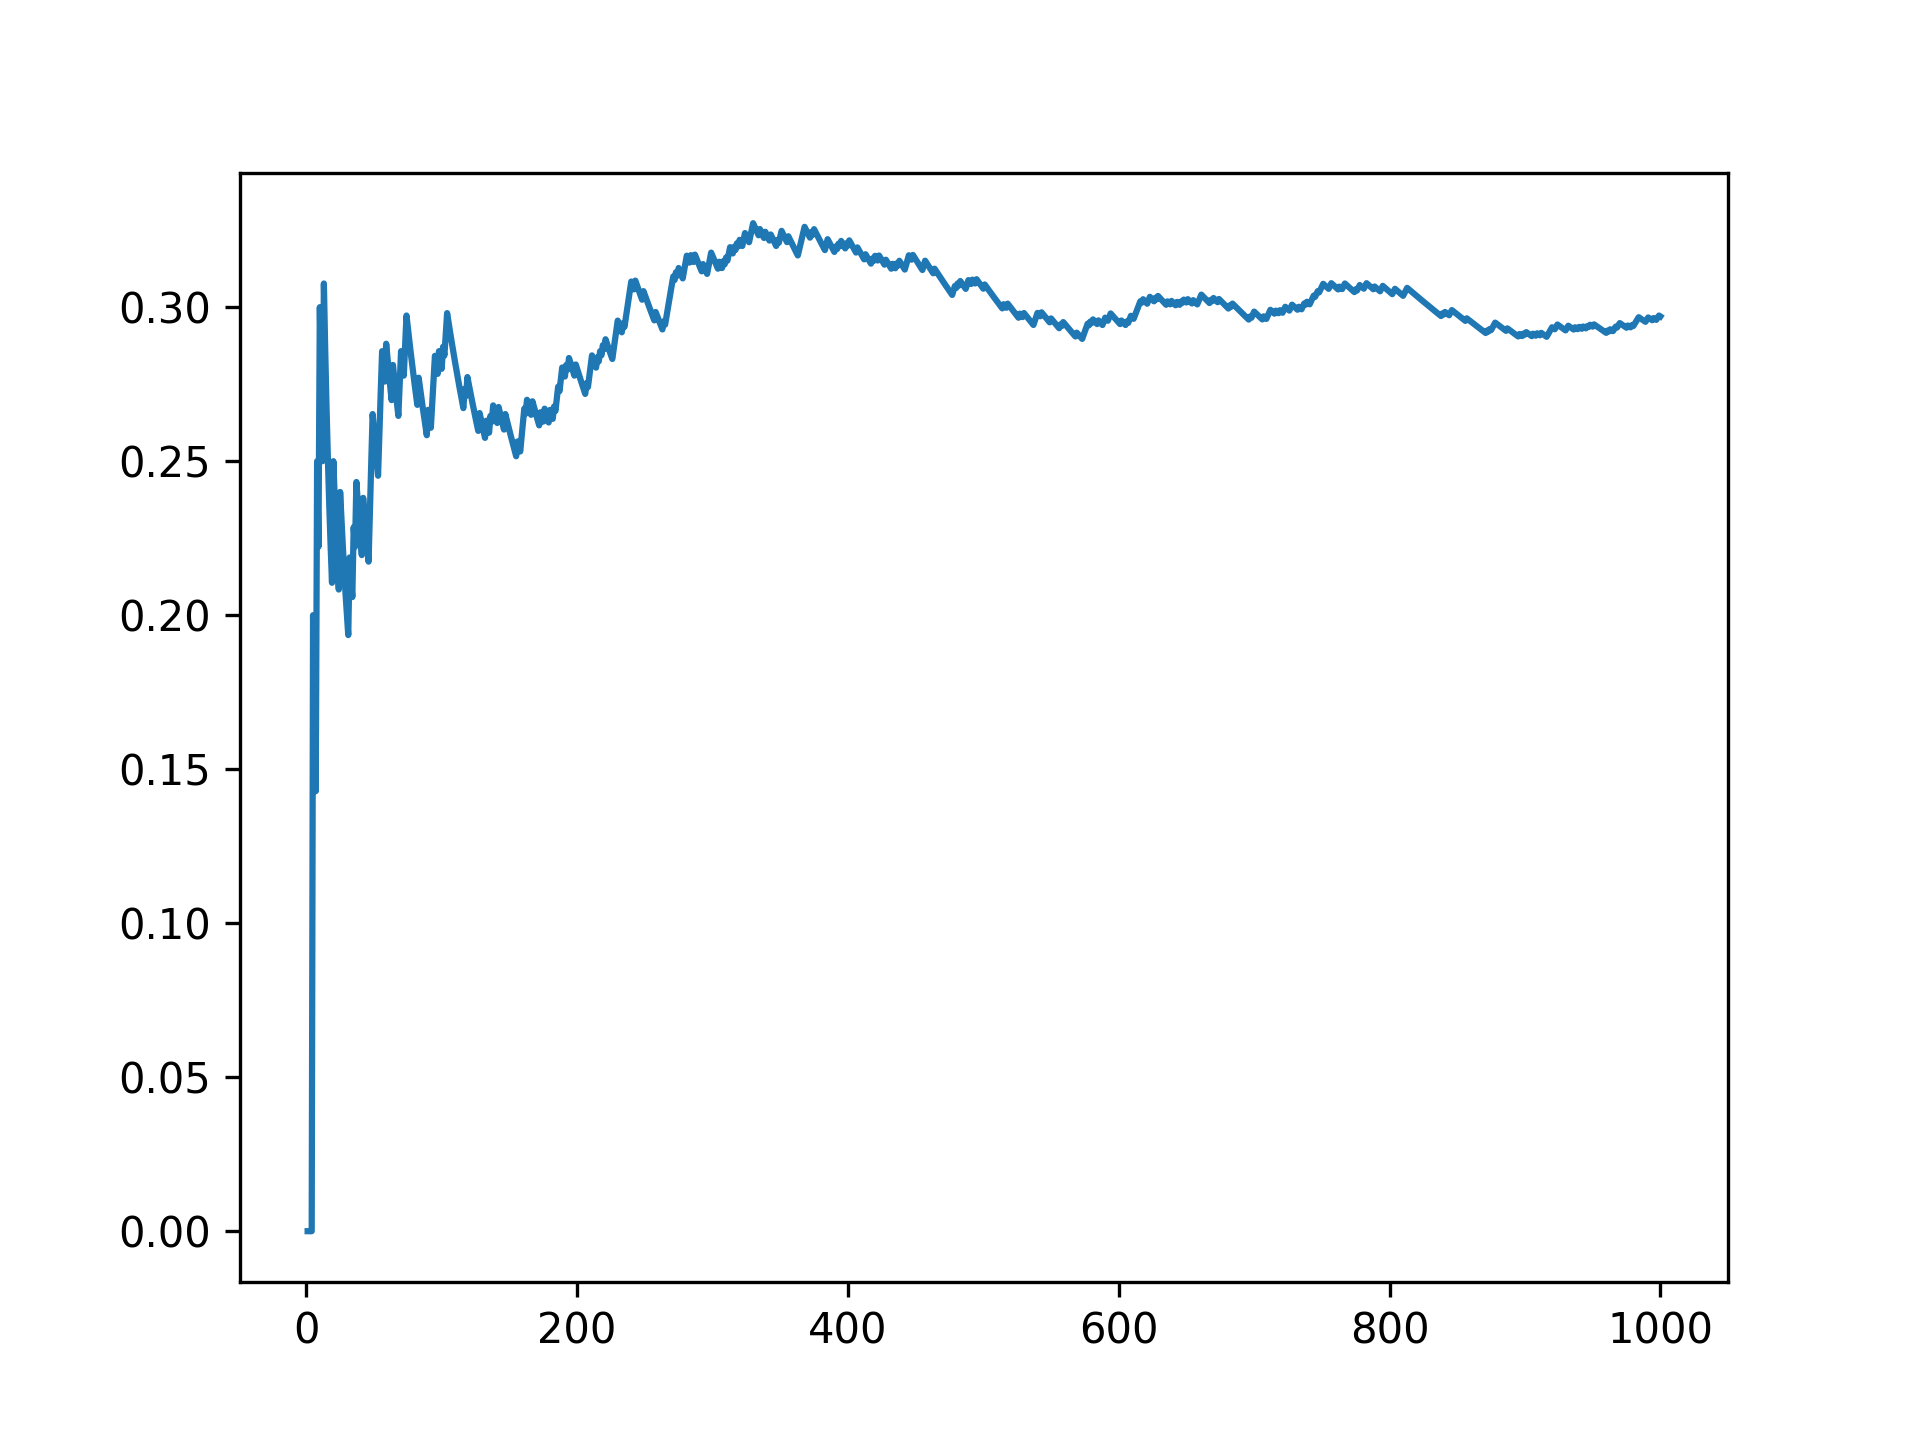
\includegraphics[width=0.45\textwidth]{1-Probability/Ex1_21-30pct_1000.png} &
			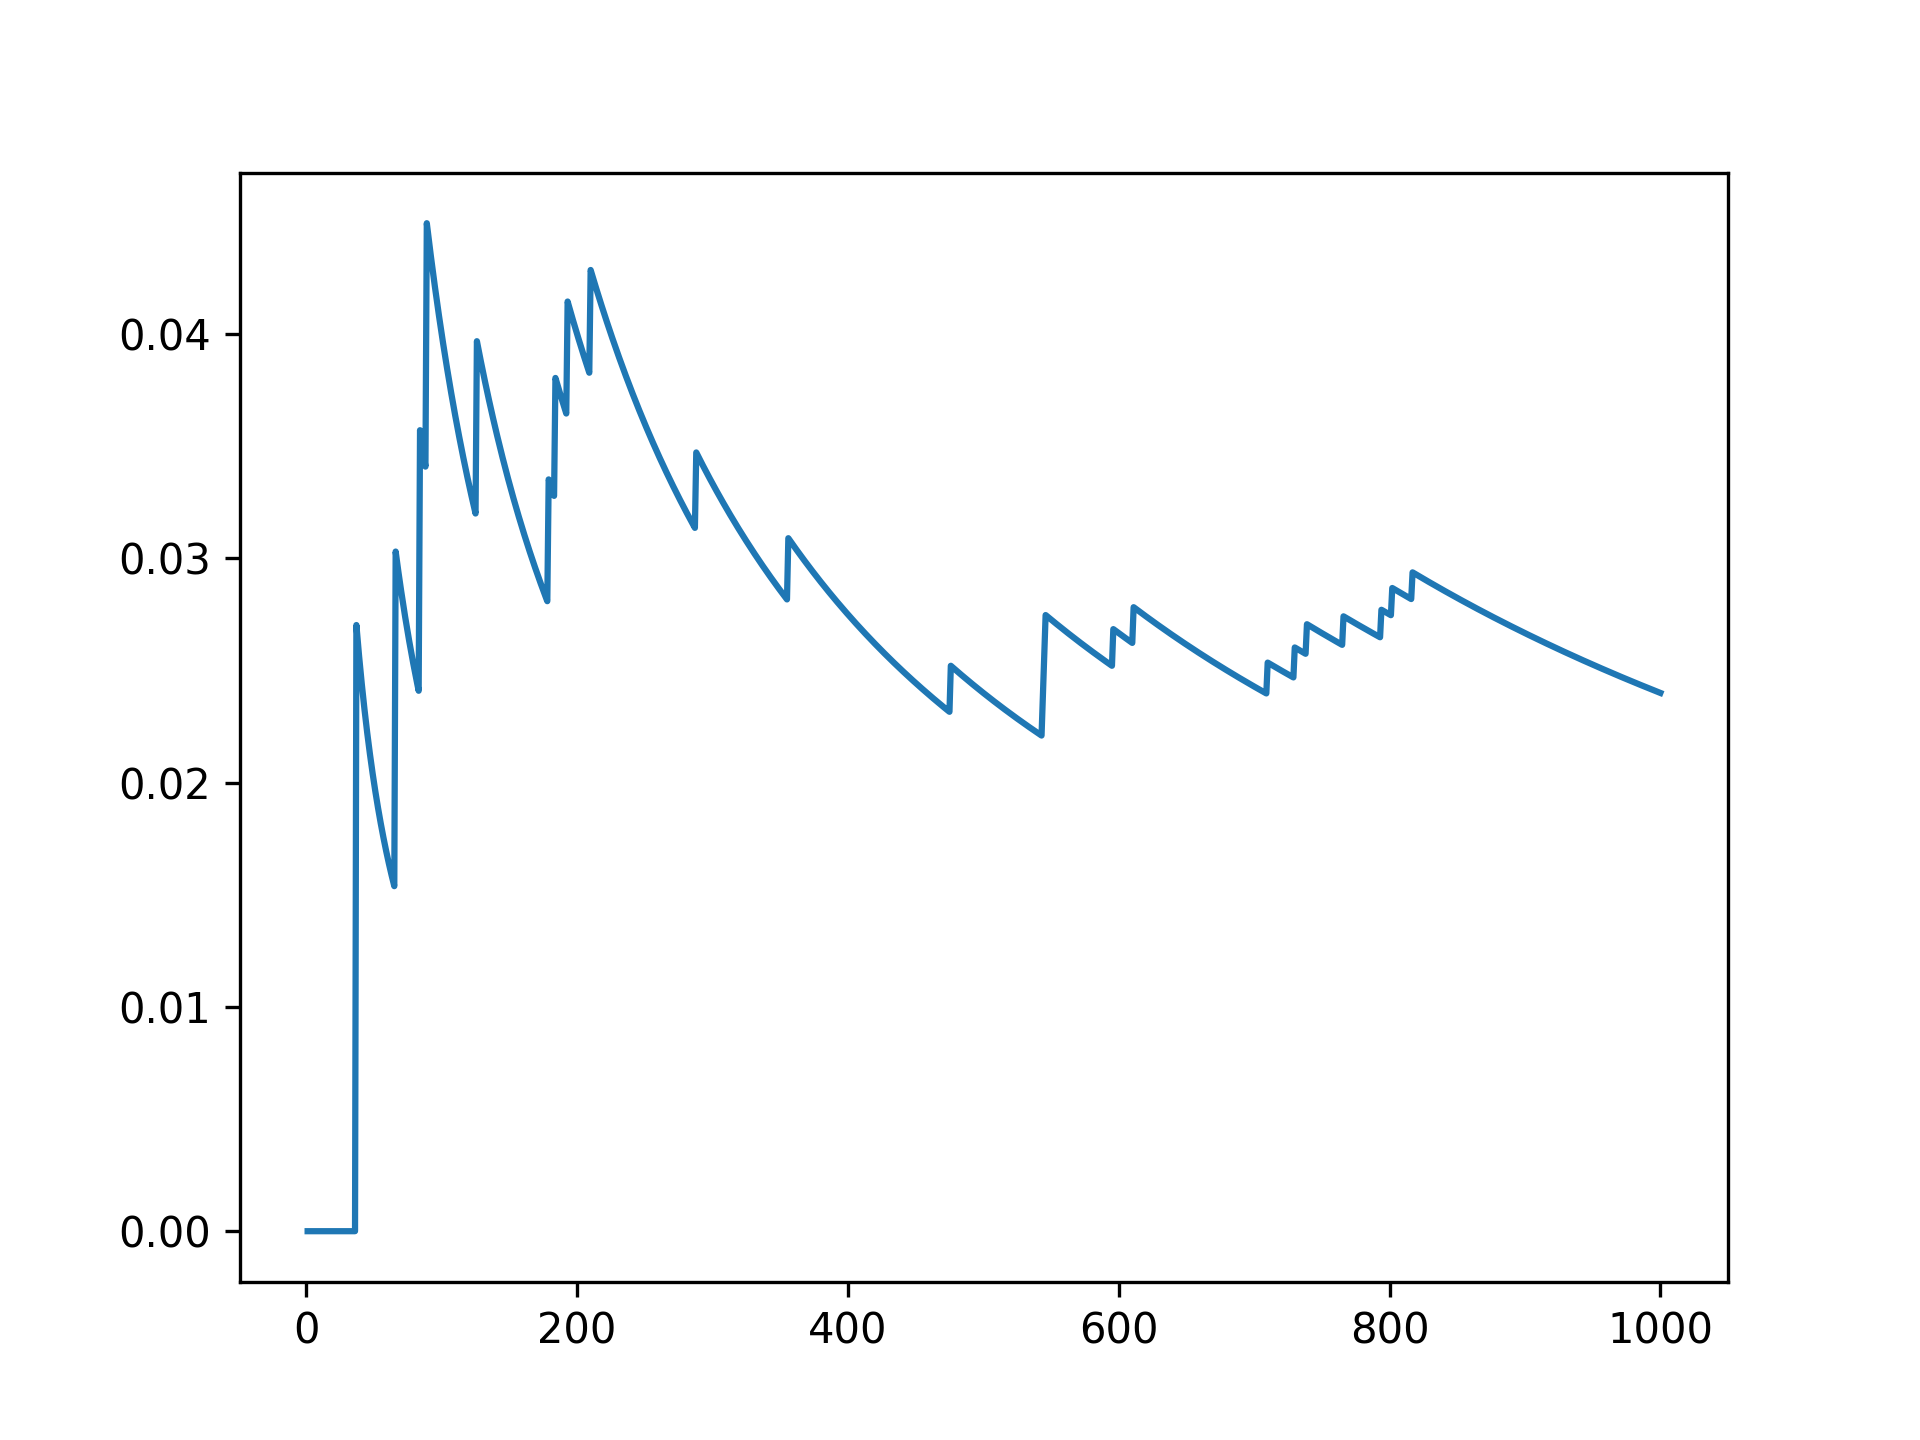
\includegraphics[width=0.45\textwidth]{1-Probability/Ex1_21-3pct_1000.png} \\
			(a) 30\% Probability & (b) 3\% Probability \\
		\end{tabular}
		\end{itemize}
	\item (Computer Experiment.) Suppose we flip a coin n times and let P denote the probability of heads. Let X be the number of heads. We call X a binomial random variable, which is discussed in the next chapter. Intuition suggests that X will be close to n p. To see if this is true, we can repeat this experiment many times and average the X values. Carry out a simulation and compare the average of the X's to n p . Try this for $p = 0.3$ and $n = 10$, $n = 100$, and $n = 1000$.
		\begin{itemize}
			\item 
\begin{minted}{python}
import numpy as np

def Ex1_22(p = 0.3, n = 1000, num_iter = 100):
    sum = 0
    for i in range(num_iter):
        rand = np.random.random(size = n)
        sum += np.sum(rand < p)

    mean = sum / num_iter
    expected = n * p
    delta = abs(mean - expected) / (expected)
    print(f"mean = {mean}, delta = {delta * 100:.2f}%")

for n in [10, 100, 1000]:
    Ex1_22(n = n)

> mean = 2.93, delta = 2.33%
> mean = 30.2, delta = 0.67%
> mean = 297.83, delta = 0.72%
\end{minted}
		\end{itemize}
	\item (Computer Experiment.) Here we will get some experience simulating conditional probabilities. Consider tossing a fair die. Let $A = \{2, 4, 6\}$ and $B = \{1, 2, 3, 4\}$. Then, $P(A) = 1/2$, $P(B) = 2/3$ and $P(AB) = 1/3$. Since $P(AB) = P(A)P(B)$, the events $A$ and $B$ are independent. Simulate draws from the sample space and verify that $\hat{P}(AB) = \hat{P}(A)\hat{P}(B)$ where $\hat{P}(A)$ is the proportion of times $A$ occurred in the simulation and similarly for $\hat{P}(AB)$ and $\hat{P}(B)$. Now find two events $A$ and $B$ that are not independent. Compute $\hat{P}(A)$,$\hat{P}(B)$ and $\hat{P}(AB)$. Compare the calculated values to their theoretical values. Report your results and interpret.
	\begin{itemize}
		\item
\begin{minted}{python}
import numpy as np

labels = ['P(A)', 'P(B)', 'P(A, B)', 'P(A)P(B)', 
          'P(A, B) - P(A)P(B)']
pct_str = lambda x : f"{x * 100:.2f}%"

def Ex1_23_helper(probabilities):
    for label, prob in zip(labels, probabilities):
        print(f"\t{label}: {pct_str(prob)}")

def Ex1_23(A, B, n = 10000):
    cap = A.intersection(B)

    # rand does [) so I need to increment high to get 6
    rand = np.random.randint(low = 1, high = 6 + 1, size = n)
    prob_A = sum(np.isin(rand, list(A))) / n
    prob_B = sum(np.isin(rand, list(B))) / n
    prob_cap = sum(np.isin(rand, list(cap))) / n

    prob_prod = prob_A * prob_B

    probabilities = [prob_A, prob_B, prob_cap, prob_prod,
                     prob_cap - prob_prod]

    print("Experimental Values")
    Ex1_23_helper(probabilities)

A, B = {2, 4, 6}, {1, 2, 3, 4}
print(f"A = {A}, B = {B}, AB = {A.intersection(B)}")
print("Theoretical Values")
Ex1_23_helper([1/2, 2/3, 1/3, 1/3, 0])
Ex1_23(A, B)
print()

A, B = {1, 2, 3}, {3, 4, 5, 6}
print(f"A = {A}, B = {B}, AB = {A.intersection(B)}")
print("Theoretical Values")
Ex1_23_helper([1/2, 2/3, 1/6, 1/3, -1/6])
Ex1_23(A, B)

> A = {2, 4, 6}, B = {1, 2, 3, 4}, AB = {2, 4}
> Theoretical Values
> 	P(A): 50.00%
> 	P(B): 66.67%
> 	P(A, B): 33.33%
> 	P(A)P(B): 33.33%
> 	P(A, B) - P(A)P(B): 0.00%
> Experimental Values
> 	P(A): 50.18%
> 	P(B): 67.42%
> 	P(A, B): 33.70%
> 	P(A)P(B): 33.83%
> 	P(A, B) - P(A)P(B): -0.13%
> 
> A = {1, 2, 3}, B = {3, 4, 5, 6}, AB = {3}
> Theoretical Values
> 	P(A): 50.00%
> 	P(B): 66.67%
> 	P(A, B): 16.67%
> 	P(A)P(B): 33.33%
> 	P(A, B) - P(A)P(B): -16.67%
> Experimental Values
> 	P(A): 50.20%
> 	P(B): 66.30%
> 	P(A, B): 16.50%
> 	P(A)P(B): 33.28%
> 	P(A, B) - P(A)P(B): -16.78%
\end{minted}
		\end{itemize}
\end{enumerate}

\subsection{Random Variables}
\begin{enumerate}
	\item Show that
	$$
	P(X = x) = F(x^+) - F(x^-).
	$$
		\begin{itemize}
			\item Note that $(\infty, x)$ and $\{x\}$ are disjoint as such
			$$
			P(X \leq x) = P(X < x) + P(X = x).
			$$
			This allows us to calculate:
			$$
			\begin{aligned}
			P(X = x) &= P(X \leq x) - P(X < x) \\
			&= F(x) - P(X < x) \\
			&= F(x) - \lim_{\varepsilon \searrow 0} P(X \leq x - \varepsilon) \\
			&= F(x) - \lim_{y \searrow x} P(X \leq y) \\
			&= F(x) - \lim_{y \searrow x} F(y) \\
			&= F(x^+) - F(x^-),
			\end{aligned}
			$$
			where we have used that $F(x) = F^+(x)$ by definition of CDFs.
		\end{itemize}
	\item Let $X$ be such that $P(X = 2) = P(X = 3) = 1 / 10$ and $P(X = 5) = 8 / 10$. Plot the CDF $F$. Use $F$ to find $P(2 < X \leq 4.8)$ and $P(2 \leq X \leq 4.8)$.
		\begin{itemize}
			\item
			\begin{minted}{python}
import numpy as np
import matplotlib.pyplot as plt

def Ex2_2(draw = True, save = False):
    x = np.arange(start=0, stop = 6, step = 0.2)
    F = (x >= 2) * 0.1 + (x >= 3) * 0.1 + (x >= 5) * 0.8
    #plt.step(x, F, where='post')

    if save:
        plt.savefig("Ex2_2.png")
    if draw:
        plt.show()

    right = np.where(abs(x - 4.8) < 0.1)[0]
    left = np.where(abs(x - 2) < 0.1)[0]
    print("P(2 <  X <= 4.8) = ", (F[right] - F[left])[0])
    print("P(2 <= X <= 4.8) = ", (F[right] - F[left - 1])[0])

Ex2_2(draw = False, save = False)

> P(2 <  X <= 4.8) =  0.1
> P(2 <= X <= 4.8) =  0.2
			\end{minted}
			\begin{center}
				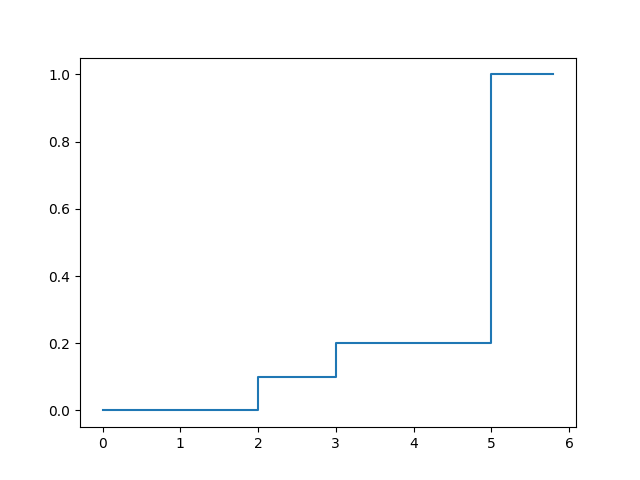
\includegraphics[width=\linewidth]{2-Random_Variables/Ex2_2.png}
			\end{center}
		\end{itemize}
	\item Prove Lemma 2.15.
	\item Let $X$ have probability density function
	$$
		f(x) = 
	\begin{cases} 
	\frac{1}{4} & \text{if } 0 < x < 1 \\
	\frac{3}{8} & \text{if } 3 < x < 5 \\
	0 & \text{otherwise}
	\end{cases}
	$$
		\begin{enumerate}
			\item Find the cumulative distribution function of $X$.
				\begin{itemize}
					\item We can obtain the CDF $F$ of $f$ by integration:
					$$
					F(t) := \int_{-\infty}^t f(x) dx,
					$$
					For $t \leq 0$ we have $F(t) = 0$. Let $t \in (0, 1)$ then
					$$
					F(t) = \int_0^t \frac{1}{4} dx = \frac{t}{4}.
					$$
					For $t \in [1, 3]$ we have
					$$
					F(t) = \int_0^1 f(x) dx = \frac{1}{4}.
					$$
					Now let $t \in (3, 5)$ then
					$$
					\begin{aligned}
					F(t) &= \int_0^1 f(x) dx + \int_3^t f(x) dx \\
					&= \frac{1}{4} + (t - 3) \frac{3}{8}.
					\end{aligned}
					$$
					And for $t \geq 5 : F(t) = 1$. In total this shows that
					$$
					F(t) = 
					\begin{cases} 
					0, & \text{if } t \leq 0, \\
					\frac{t}{4}, & \text{if } t \in (0, 1), \\
					\frac{1}{4}, & \text{if } t \in [1, 3], \\
					\frac{1}{4} + \frac{3}{8}(t - 3), & \text{if } t \in (3, 5), \\
					1, & \text{if } t \geq 5.
					\end{cases}
					$$
				\end{itemize}
			\item Let $Y = 1 / X$. Find the probability density function $f_Y(y)$ for $Y$. Hint. Consider three cases: $\frac{1}{5} \leq y \leq \frac{1}{3}$, $\frac{1}{3} \leq y \leq 1$, and $y \geq 1$.
				\begin{itemize}
					\item First of all, note that $0 < X < 5$, as such $\frac{1}{5} < Y$. This means that
					$$
					P(Y \leq y) = P\left(\frac{1}{5} < Y \leq y \right)
					$$
					Now suppose $y \in \left(\frac{1}{5}, \frac{1}{3} \right)$, then
					$$
					P\left(Y \leq y\right) = P\left( \frac{1}{5} < Y \leq y \right)
					$$
					By definition
					$$
					\frac{1}{5} < Y \leq y \iff \frac{1}{y} \leq \frac{1}{Y} < 5 \iff \frac{1}{y} \leq X < 5.
					$$
					Then
					$$
					P\left(Y \leq y\right) = P\left(\frac{1}{y} \leq X < 5\right) = F(5) - F\left( \frac{1}{y} \right).
					$$
					This can then be computed by noting that $F(5) = 1$ and $F(1 / y) = \frac{1}{4} + \frac{3}{8}(\frac{1}{y} - 3)$.

					For $\frac{1}{3} \leq y \leq 1$ we have
					$$
					P\left(Y \leq y\right) = F(3) - F\left(\frac{1}{y}\right)
					$$
					and this is equal to $\frac{1}{4}$. For $y \geq 1$ we have $\frac{1}{y} \leq 1$ and
					$$
					\frac{1}{4} - \frac{1}{4y}.
					$$
					In total this means [TODO: Finish this].
				\end{itemize}
		\end{enumerate}
	\item Let $X$ and $Y$ be discrete random variables. Show that $X$ and $Y$ are independent if and only if $f_{X, Y}(x, y) = f_X(x)f_Y(y)$ for all $x$ and $y$.
	\item Let $X$ have distribution $F$ and density function $f$ and let $A$ be a subset of $\mathbb{R}$. Denote by $I_A(x)$ the indicator function for $A$. Let $Y = I_A(X)$. Find an expression for the cumulative distribution of $Y$. Hint: first find the probability mass function for $Y$.
		\begin{itemize}
			\item Denote the CDF of $Y$ by $G$. Note that $Y$ either takes $0$ or $1$ as its value. The PDF $g$ of $Y$ is $g(t) = 1$ if $X(t) \in A$ and $0$ else. This means that the CDF for $y < 0$ is just $0$, for $0 \leq y < 1$, $G(y) = P(X \in A)$ and $G(y) = 1$ for all $y \geq 1$. Note that
			$$
			P(X \notin A) = 1 - P(X \in A) = 1 - \int_A f(x) dx.
			$$
		\end{itemize}
	\item Let $X$ and $Y$ be independent and suppose that each has a $\operatorname{Uniform}(0, 1)$ distribution. Let $Z = \min\{X, Y\}$. Find the density $f_Z(z)$ for $Z$. Hint: It might be easier to first find $P(Z > z)$.
		\begin{itemize}
			\item By definition we have 
			$$
			P(Z > z) = P(\min{X, Y} > z) = P(X > z, Y > z),$$
			because $X$ and $Y$ are independent it follows that this is equal to $P(X > z)P(Y > z)$, because both of those have the same distribution those two probabilities are the same:
			$$
			P(X > z)P(Y > z) = P(X > z)^2 = (1 - P(X \leq z))^2 = (1 - z)^2.
			$$
			As such
			$$
			P(Z \leq z) = 1 - p(Z > z) = 1 - (1 - z)^2 = 2z - z^2.
			$$
			Differentiating this yields the PDF
			$$
			f_Z(z) = 2 - 2z.
			$$
		\end{itemize}
	\item Let $X$ have CDF $F$. Find the CDF of $X^+ = \max{0, X}$.
		\begin{itemize}
			\item Note that for $y \leq 0$ we have $P(X^+ \leq y) = F(0)$. For $x > 0$ we have
			$$
			\begin{aligned}
			F(X^+ \leq x) &= F(X^+ \leq 0) + P(0 < X^+ \leq x) \\
			&= F(0) + P(0 < X \leq x) \\
			&= F(0) + F(x) - F(0) \\
			&= F(x).
			\end{aligned}
			$$
		\end{itemize}
	\item Let $X \sim \operatorname{Exp}(\beta)$. Find $F(x)$ and $F^{-1}(q)$.
		\begin{itemize}
			\item The PDF of $f$ is given by $f(x) = \frac{1}{\beta} e^{- x / \beta}$ for $x > 0$ and $0$ for $x \leq 0$. We obtain the CDF of $X$ by integrating. For $t \leq 0$ we have F(t) and for $t > 0$
			$$
			F(t) = \int_{-\infty}^t f(x) dx = \int_0^t \frac{1}{\beta} e^{-x / \beta} dx.
			$$
			Recall that the antiderivative of $e^{Ax}$ is $\frac{1}{A} e^{Ax}$ as such
			$$
			\begin{aligned}
			F(t) &= \left. \frac{1}{\beta} \frac{1}{-\frac{1}{\beta}} e^{-x / \beta} \right|_{x = 0}^{x = t} \\
			&= - e^{-t / \beta} + e^{-0 / \beta}.
			\end{aligned}
			$$
			As such
			$$
			F(t) = 1 - e^{-t / \beta}.
			$$
			Per definition $F^{-1}(q) = \inf \{x : F(x) > q\}$ for $q \in [0, 1]$. For a continuous and monotone increasing function $F$ (which is the case for the exponential distribution) this is simply
			$$
			x = F^{-1}(q).
			$$
			As such we want to solve $F(x) = q$ for $x$, this is a straightforward computation:
			$$
			\begin{aligned}
			&& q &= 1 - e^{-x / \beta} \\
			\iff&& e^{-t / \beta} &= 1 - q \\
			\iff&& -t/\beta &= \log(1 - q) \\
			\iff&& t &= -\beta \log(1 - q).
			\end{aligned}
			$$
		\end{itemize}
	\item Let $X$ and $Y$ be independent. Show that $g(X)$ is independent of $h(Y)$ where $g$ and $h$ are functions.
	\item Suppose we toss a coin once and let $p$ be the probability of heads. Let $X$ denote the number of heads and let $Y$ denote the number of tails.
		\begin{enumerate}
			\item Prove that $X$ and $Y$ are dependent.
				\begin{itemize}
					\item Suppose $p \in (0, 1)$ then $P(X = 1) = p$ and $P(Y = 1) = 1 - p$ but $P(X = 1, Y = 1) = 0$, as such $X$ and $Y$ can't be independent.
				\end{itemize}
			\item Let $N \sim \operatorname{Poisson}(\lambda)$ and suppose we toss a coin $N$ times. Let $X$ and $Y$ be the number of heads and tails. Show that $X$ and $Y$ are independent.
		\end{enumerate}
	\item Prove Theorem 2.33
	\item Let $X \sim \mathcal{N}(0, 1)$ and let $Y = e^X$.
		\begin{enumerate}
			\item Find the PDF for $Y$. Plot it.
				\begin{itemize}
					\item Note that $P(Y \leq t) = P(e^X \leq t) = P(X \leq \log(t))$. We can obtain the PDF $g$ of $Y$ by differentiation:
					$$
					\frac{d}{dt} F(\log(t)) = \frac{1}{\sqrt{2\pi} t} e^{- \frac{\log(t)^2}{2}}.
					$$
					\begin{minted}{python}
import numpy as np
import matplotlib.pyplot as plt

x = np.arange(start = 0.01, stop = 7, step = 0.01)
y = np.exp(- np.log(x)**2 * 0.5) * 0.5 / x
y = y / np.sqrt(2 * np.pi)
plt.plot(x, y)

plt.savefig('Ex2_13a.png')
					\end{minted}
					\begin{center}
						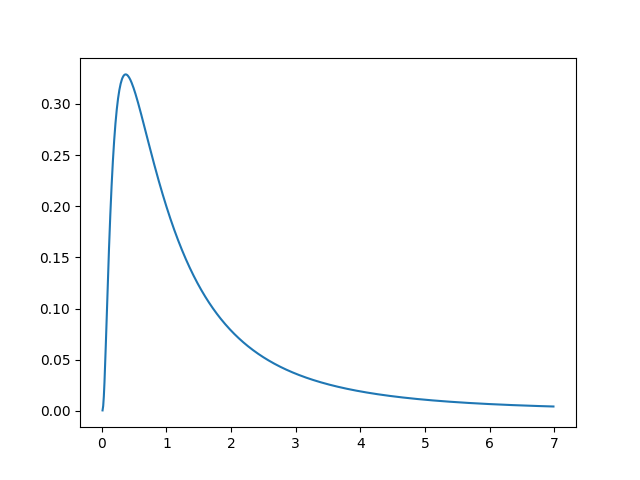
\includegraphics[width=\linewidth]{2-Random_Variables/Ex2_13a.png}
					\end{center}
				\end{itemize}
			\item (Computer Experiment) Generate a vector $x = (x_1, \dots, x_{10000})$ consisting of $10000$ random standard Normals. Let $y = (y_1, \dots, y_{10000})$ where $y_i = e^{x_i}$. Draw a histogram of $y$ and compare it to the PDF you found in part $(a)$.
				\begin{itemize}
					\item
					\begin{minted}{python}
import numpy as np
import matplotlib.pyplot as plt

x = np.random.randn(10000)
y = np.exp(x)

plt.hist(y, bins=50)
plt.savefig('Ex2_13b.png', dpi=300)
					\end{minted}
					\begin{center}
						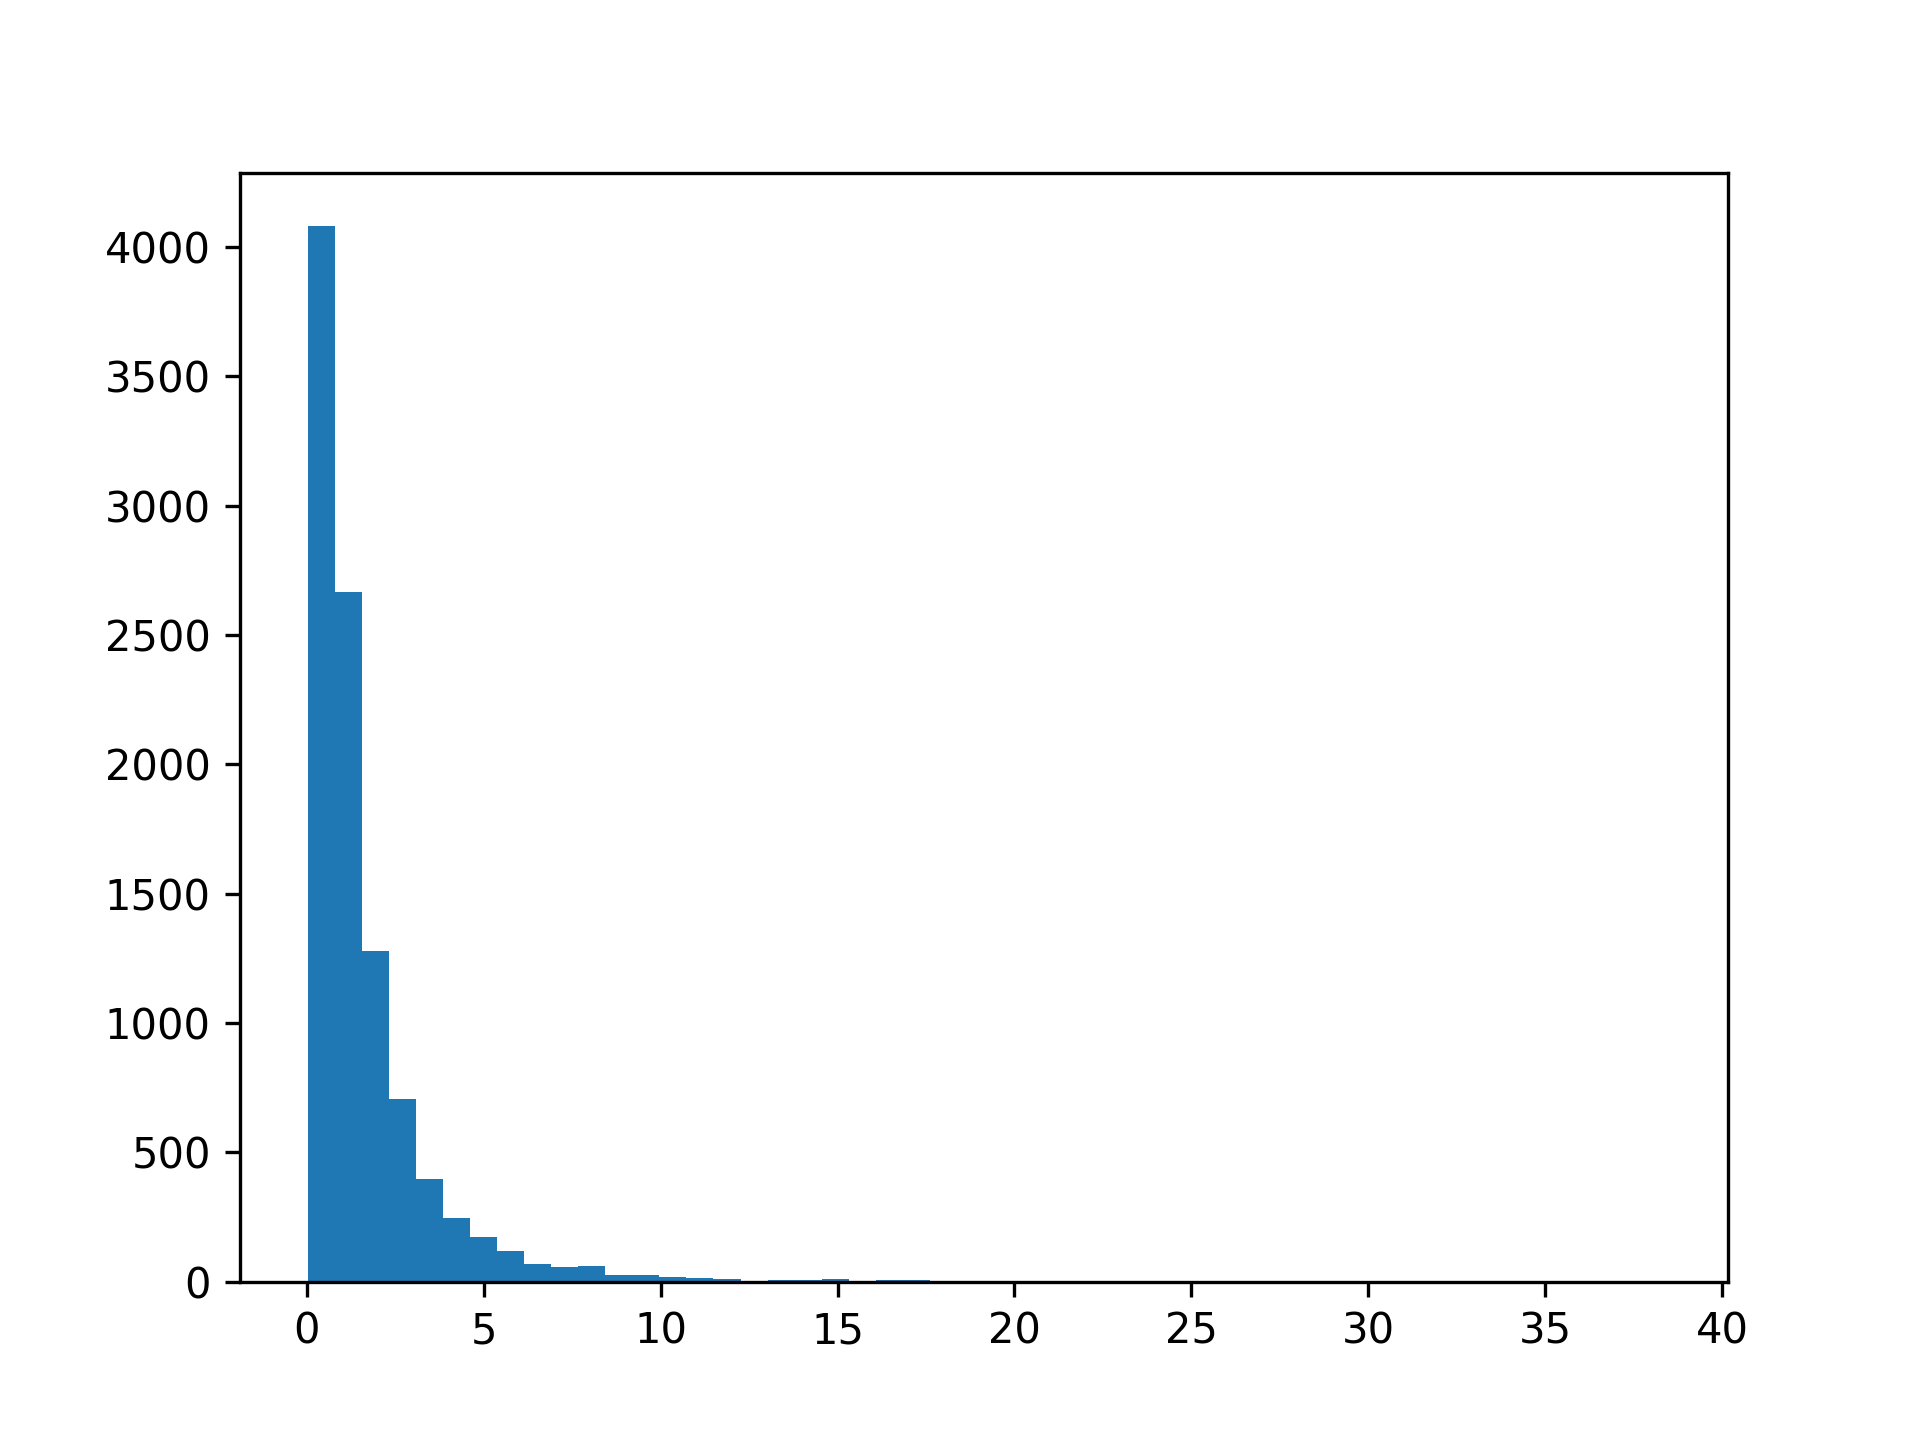
\includegraphics[width=\linewidth]{2-Random_Variables/Ex2_13b.png}
					\end{center}
				\end{itemize}
		\end{enumerate}
	\item Let $(X, Y)$ be uniformly distributed on the unit disk $\{(x, y) : x^2 + y^2 \leq 1\}$. Let $R = \sqrt{X^2 + Y^2}$. Find the CFD and PDF of $R$.
	\item Let $X$ have a continuous, strictly increasing CDF $F$. Let $Y = F(X)$. Find the density of $Y$. This is called the probability integral transform. Now, let $U \sim \operatorname{Uniform}(0,1)$ and let $X = F^{-1}(U)$. Show that $X \sim F$. Now write a program that takes Uniform $(0,1)$ random variables and generates random variables from an Exponential $(\lambda)$ distribution.
	\item Let $X \sim \operatorname{Poisson}(\lambda)$ and $Y \sim \operatorname{Poisson}(\mu)$ and assume that $X$ and $Y$ are independent. Show that the dstribution of $X$ given that $X + Y = n$ is $\operatorname{Binomial}(n, \pi)$ where $\pi = \frac{\lambda}{\lambda + \mu}$.
	Hint 1: You may use the following fact: If $X \sim \operatorname{Poisson}(\lambda)$ and $Y \sim \operatorname{Poisson}(\mu)$, and $X$ and $Y$ are independent, then $X + Y \sim \operatorname{Poisson}(\lambda + \mu)$.
	Hint 2: Note that $\{X = x, X + Y = n\} = \{X = x, Y = n - x\}$.
		\begin{itemize}
			\item Recall that
			$$
			P(X = x|X + Y = n) = \frac{P(X = x, X + Y = n)}{P(X + Y = n)}.
			$$
			By the first hint $P(X + Y = n) = \frac{(\lambda + \mu)^n}{n!} e^{-\lambda -\mu}$. Using the second hint we obtain
			$$
			P(X = x, X + Y = n) = P(X = x, Y = n - x),
			$$
			using the independence of $X$ and $Y$ this becomes
			$$
			P(X = x)P(Y = n - x) = \frac{\lambda^x}{x!} e^{-\lambda} \frac{\mu^{n - x}}{(n - x)!}e^{-\mu}.
			$$
			Combining everything then yields
			$$
			\begin{aligned}
			P(X = x|X + Y = n) &= \frac{\frac{\lambda^x}{x!} e^{-\lambda} \frac{\mu^{n - x}}{(n - x)!}e^{-\mu}}{\frac{(\lambda + \mu)^n}{n!} e^{-\lambda-\mu}} \\
			&= \frac{\lambda^x \mu^{n - x}}{(\lambda + \mu)^n} \frac{n!}{x! (n - x)!}
			&= \frac{\lambda^x \mu^{n - x}}{(\lambda + \mu)^n} \binom{n}{x}.
			\end{aligned}
			$$
			Note that if $Z \sim \operatorname{Bin}\left(n, \frac{\lambda}{\lambda + \mu}\right)$ then
			$$
			\begin{aligned}
			P(Z = k) &= \binom{n}{k} \left(\frac{\lambda}{\lambda + \mu}\right)^k \left( 1 - \frac{\lambda}{\lambda + \mu} \right)^{n - k} \\
			&= \binom{n}{k} \left(\frac{\lambda}{\lambda + \mu}\right)^k \left( \frac{\mu}{\lambda + \mu}\right)^{n - k} \\
			&= \frac{n!}{k!(n - k)!} \left(\frac{\lambda}{\lambda + \mu}\right)^k \left( \frac{\mu}{\lambda + \mu}\right)^{n - k}.
			\end{aligned}
			$$
			As such we have shown that $X|X + Y = n \sim \operatorname{Bin}\left(n, \frac{\lambda}{\lambda + \mu}\right)$.
		\end{itemize}
	\item 
	\item 
	\item Prove formula (2.12)
	\item Let $X, Y \sim \operatorname{Uniform}(0, 1)$ be independent. Find the PDF for $X - Y$ and $X / Y$.
	\item Let $X_1, \dots, X_n \sim \operatorname{Exp}(\beta)$ be iid. Let $Y = \max\{X_1, \dots, X_n\}$. Find the PDF of $Y$. Hint: $Y \leq y$ if and only if $X_i \leq y$ for all $i = 1, \dots, n$.
		\begin{itemize}
			\item To compute the PDF of $Y$, we first determine the CDF of $Y$:
			$$
			\begin{aligned}
			P(Y \leq y) &= P(X_1 \leq y, \dots, X_n \leq y) \\
			&\overset{1}{=} \prod_{i = 1}^n P(X_i \leq y) \\
			&\overset{2}{=} P(X_1 \leq y)^n \\
			&= \left(1 - e^{- \frac{- y}{\beta}}\right),
			\end{aligned}
			$$
			where we have used (1) that the $X_i$ are independent and (2) that they are identically distributed. Differentiating this with respect to $y$ yields
			$$
			\frac{d}{dy} P(Y \leq y) = n (1 - e^{- y / \beta})^{n - 1} \frac{1}{\beta} e^{- y / \beta}.
			$$
		\end{itemize}
\end{enumerate}

\subsection{Expectation}
\begin{enumerate}
	\item 
	\item 
	\item
	\item 
	\item
	\item Prove Theorem 3.6 for discrete random variables
	\item 
	\item Prove Theorem 3.17
	\item (Computer Experiment) Let $X_1, X_2, \dots, X_n$ be $\mathcal{N}(0, 1)$ random variables and let
	$$
	\overline{X}_n = \frac{1}{n} \sum_{i = 1}^n X_i.
	$$
	Plot $\overline{X}_n$ versus $n$ for $n = 1, \dots, 10000$. Repeat for $X_1, X_2, \dots, X_n \sim \operatorname{Cauchy}$. Explain why there is such a difference.
		\begin{itemize}
			\item
			\begin{minted}{python}
import numpy as np
import matplotlib.pyplot as plt

n = 10000

samples = np.random.normal(size = n)
samples_cauchy = np.random.standard_cauchy(size = n)

x = (np.arange(n) + 1)

mean = np.cumsum(samples) / x
mean_cauchy = np.cumsum(samples_cauchy) / x

plt.plot(x, mean, label='Normal Mean')
plt.plot(x, mean_cauchy, label='Cauchy Mean')

plt.legend(loc='upper right')

plt.savefig("Ex3_9.png")
			\end{minted}
			\begin{center}
				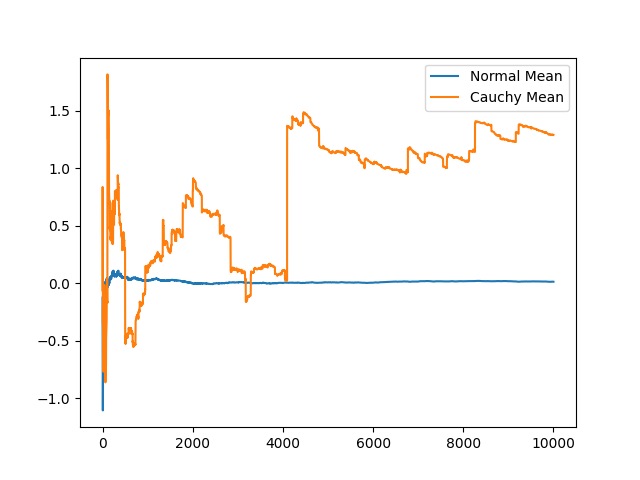
\includegraphics[width=\linewidth]{3-Expectation/Ex3_9.png}
			\end{center}
		\end{itemize}
	\item 
	\item (Computer Experiment: Simulating the Stock Market). Let $Y_1, Y_2, \dots$ be independent random variables such that $P(Y_i = 1) = P(Y_i = -1) = \frac{1}{2}$. Let $X_n = \sum_{i = 1}^n Y_i$. Think of $Y_i = 1$ as "the stock market increased by one dollar", $Y_i = -1$ as "the stock market decreased by one dollar", and $X_n$ as the value of the stock on day $n$.
		\begin{enumerate}
			\item Find $E(X_n)$ and $Var(X_n)$.
				\begin{itemize}
					\item By linearity $E(X_n) = \sum_{i = 1}^n E(Y_i) = \sum_{i = 1}^n (-1)\frac{1}{2} + (1) \frac{1}{2} = 0.$ Note that $E(X_n)^2 = 0$, as such $Var(X_n) = E(X_n^2)$. To calculate this note that
					$$
					X_n^2 = \left( \sum_{i = 1}^n Y_i \right)^2 = \sum_{i = 1}^n Y_i^2 + 2 \sum_{i < j} Y_i Y_j.
					$$
					Because $Y_i \in \{-1, 1\}$ it follows that $E(Y_i^2) = 1$ and as such
					$$
					E(X_n^2) = n + 2 \sum_{i < j} E(Y_i Y_j) = n + 2 \sum_{i < j} P(Y_i Y_j = +1) - P(Y_i Y_j = -1).
					$$
					Note that $Y_i Y_j = 1$ if and only if $(Y_i, Y_j) \in \{(1, 1), (-1, -1)\}$ and $Y_i Y_j = -1$ if and only if $(Y_i, Y_j) \in \{(-1, 1), (1, -1)\}$, as such both of those are equally liked. In total this means that
					$$
					V(X_n) = E(X_n^2) = n.
					$$
				\end{itemize}
			\item Simulate $X_n$ and plot $X_n$ versus $n$ for $n = 1, 2, \dots, 10000$. Repeat the whole simulation several times. Notice two things. First, it's easy to "see" patterns in the sequence even though it is random. Second, you will find that the four runs look very different even though they were generated the same way. How do the calculations in (a) explain the second observation?
				\begin{itemize}
					\item
\begin{minted}{python}
import numpy as np
import matplotlib.pyplot as plt

def Ex3_11(n = 10000, draw = True, save = False, i = 0):
    # 2*0 - 1 = -1, 2 * 1 -1 = 1
    rand = 2 * np.random.randint(low = 0, high = 2, size = n) - 1

    fig, ax = plt.subplots()
    ax.plot(range(0, n), np.cumsum(rand))

    if draw:
        plt.show()

    if save:
        fig.savefig(f"Ex3_11-{i}.png")

for i in range(4):
    Ex3_11(draw = True, save = True, i = i)
\end{minted}
\begin{figure}
  \centering
  \begin{tabular}{cc}
    \begin{subfigure}{0.45\linewidth}
      \centering
      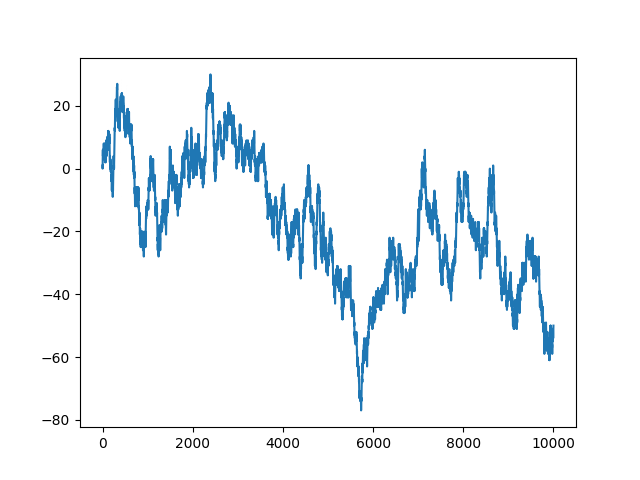
\includegraphics[width=\linewidth]{3-Expectation/Ex3_11-0.png}
      \caption{}
    \end{subfigure}
    &
    \begin{subfigure}{0.45\linewidth}
      \centering
      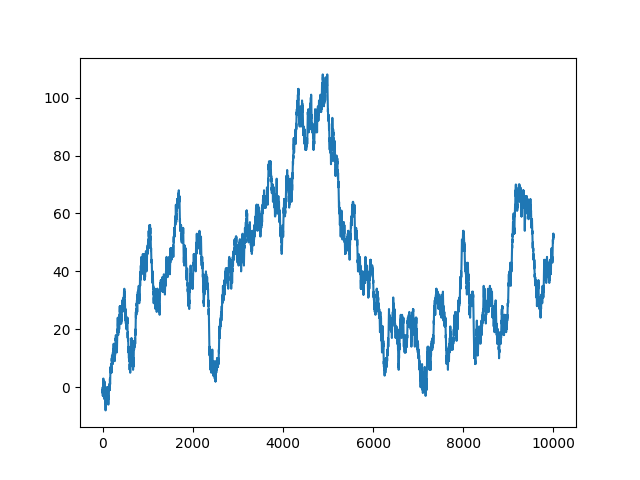
\includegraphics[width=\linewidth]{3-Expectation/Ex3_11-1.png}
      \caption{}
    \end{subfigure}
    \\
    \begin{subfigure}{0.45\linewidth}
      \centering
      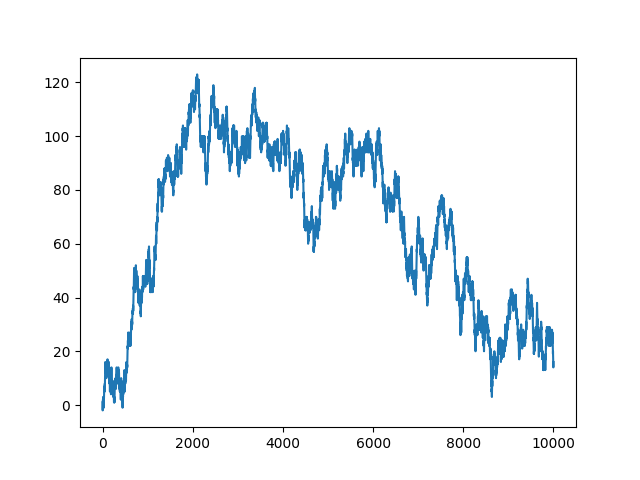
\includegraphics[width=\linewidth]{3-Expectation/Ex3_11-2.png}
      \caption{}
    \end{subfigure}
    &
    \begin{subfigure}{0.45\linewidth}
      \centering
      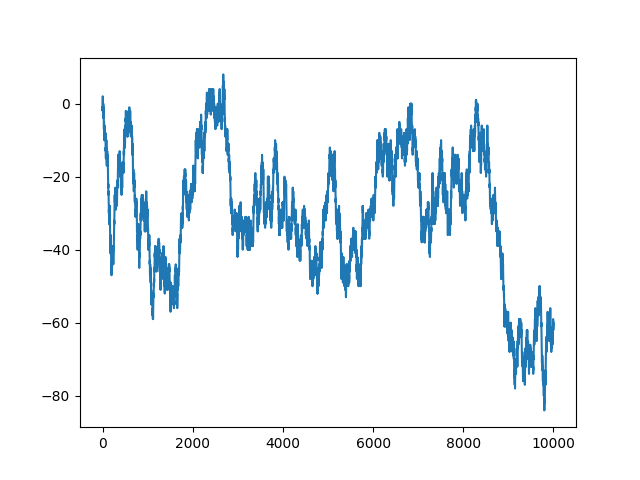
\includegraphics[width=\linewidth]{3-Expectation/Ex3_11-3.png}
      \caption{}
    \end{subfigure}
  \end{tabular}
\end{figure}
				\end{itemize}
		\end{enumerate}
	\item
\end{enumerate}

\end{document}
